% Kuber: Geometry-General Neural Surrogates for Conjugate Heat Transfer
% Compiles with pdflatex (or on Overleaf). Figures are in ../assets/sim/.
\documentclass[10pt,twocolumn]{article}
\usepackage[letterpaper,margin=0.75in]{geometry}
\usepackage{times}
\usepackage{graphicx}
\usepackage{booktabs}
\usepackage{amsmath,amssymb}
\usepackage{pifont}
\usepackage{caption}
\usepackage[hidelinks]{hyperref}
\captionsetup{font=small,labelfont=bf}
\graphicspath{{../assets/sim/}}
\setlength{\parskip}{2pt}
\pagestyle{empty}

\title{\vspace{-2em}\bfseries Kuber: Geometry-General Neural Surrogates\\ for Conjugate Heat Transfer}
\author{Shubh Jain\\ \normalsize Kuber.ai \\
\normalsize\ttfamily github.com/ShubhJain007/Kuber}
\date{\normalsize Technical Report \textperiodcentered\ 2026}

\begin{document}
\twocolumn[
\begin{@twocolumnfalse}
\maketitle
\begin{center}\itshape\small
A reproducible OpenFOAM benchmark and a surface-conditioned transformer surrogate\end{center}
\begin{abstract}\noindent
Conjugate heat transfer (CHT) --- the coupled transport of heat through a solid conductor and a
surrounding moving fluid --- governs the thermal design of heatsinks, cold plates, heat exchangers,
power electronics, and battery packs. High-fidelity CFD resolves these fields but costs minutes to
hours per geometry, prohibitive inside a design loop. We present \textbf{Kuber}, an open framework
for building neural surrogates of CHT, and \textbf{SurfaceGeoTransolver}, a geometry-general model
that predicts the full steady field $(U,T,p)$ at an arbitrary query point cloud in a sub-second. The
model couples a physics-attention transformer core with a surface-geometry encoder, so it ingests
raw boundary geometry (a surface point cloud with normals) and requires no analytic signed-distance
field, and it is conditioned on the full set of physical scalars plus a device-class flag. On the
public SIMSHIFT heatsink benchmark it attains \textbf{12.14\,K temperature RMSE} on the medium
out-of-distribution split, improving on the best previously published result (12.41\,K) while using
\textbf{no unsupervised domain adaptation}, which every reported baseline relies on. A single set of
weights spans two physically distinct device classes --- buoyancy-driven heatsinks in air and
forced-convection liquid cold plates --- and pretraining on a self-generated OpenFOAM corpus lowers
out-of-distribution error further. We additionally verify numerical soundness: the predicted
temperature gradient never exceeds the physical gradient at fin tips and corners (explosion fraction
zero, no NaN/Inf). All results are reproducible with the released code and data.
\end{abstract}
\vspace{1em}
\end{@twocolumnfalse}
]

\section{Introduction}
Thermal design is an inner loop. An engineer proposes a geometry and must know the resulting
temperature and flow field before iterating. The field is produced by solving the coupled
Navier--Stokes and energy equations across a solid and a fluid region: \emph{conjugate heat transfer}
(CHT). Finite-volume CFD solves this accurately but slowly; in our measurements a single steady case
takes a median of 22 minutes and up to nearly two hours for fine geometries. Sweeping thousands of
designs, or closing an optimization loop, is therefore dominated by solver cost.

Neural surrogates promise to amortize this cost: learn the geometry-to-field map once, then evaluate
in milliseconds. Recent operator-learning and transformer methods have made this practical for
external aerodynamics, but electronics-cooling CHT has received far less attention, has no widely used
open benchmark harness, and no shared, license-clean data-generation recipe. Two requirements make the
problem hard. First, \emph{geometry generality}: a useful surrogate must accept arbitrary CAD, which
rules out geometry encodings that presuppose an analytic shape. Second, \emph{generalization}: the
surrogate must predict geometries it never saw in training.

We make three contributions. (i) \textbf{SurfaceGeoTransolver}, a surface-conditioned physics
transformer that predicts the full 5-channel CHT field at any query point from raw boundary geometry
and physical conditioning, reaching state of the art on a public benchmark without domain adaptation.
(ii) A \textbf{reproducible data engine} generating a self-labeled OpenFOAM CHT corpus across fluids,
regimes, shapes, and two device classes, with a convergence gate and a verified mesh-convergence
protocol. (iii) An \textbf{honest evaluation harness} --- per-field normalized error, near-wall
fidelity, a numerical no-explosion proof, and a value-of-data ablation --- with released code, data,
machine-readable results, and an interactive viewer.

\begin{figure*}[t]
\centering
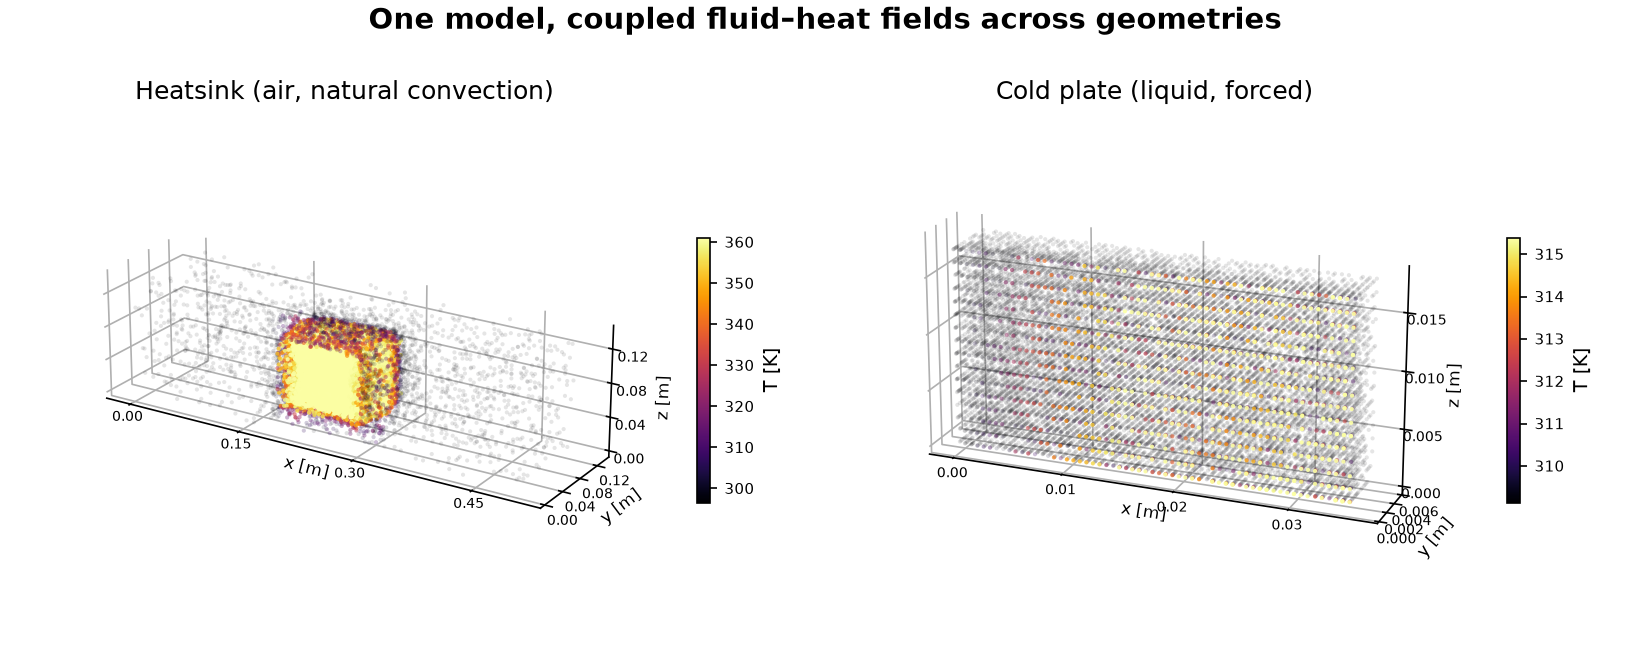
\includegraphics[width=0.98\textwidth]{hero.png}
\caption{Coupled fluid--heat fields predicted by a single model across two device classes: a heatsink
in natural-convection air (left) and a liquid-cooled cold plate (right), colored by temperature
(OpenFOAM ground truth shown).}
\label{fig:hero}
\end{figure*}

\section{Related work}
\textbf{Neural operators.} DeepONet~\cite{deeponet} and the Fourier Neural Operator~\cite{fno}
established learning maps between function spaces; GINO~\cite{gino} extended operator learning to
large 3D geometries. These are strong on fixed domains but do not natively consume arbitrary boundary
geometry with per-node queries. \textbf{Transformer PDE solvers.} Transolver~\cite{transolver}
introduced physics attention over learned slices; UPT~\cite{upt} and the anchored/branched
variant~\cite{abupt} scale transformer surrogates to industrial CFD. Our core builds on the
GeoTransolver implementation in NVIDIA PhysicsNeMo~\cite{physicsnemo}; our contribution is the
surface-conditioning branch and the CHT-specific conditioning and training recipe.
\textbf{Geometry.} Signed-distance fields are data-efficient when an analytic shape exists, but none
exists for arbitrary CAD; following the surface branch of AB-UPT~\cite{abupt} we encode the boundary
directly as a point cloud with normals. \textbf{Spectral fidelity.} One-shot regression is spectrally
biased; PDE-Refiner~\cite{pderefiner} restores high-frequency content, which we adopt as an optional
head. \textbf{Benchmarks.} SIMSHIFT~\cite{simshift} is a public benchmark for distribution shift in
engineering simulation; we use its heatsink task as our primary evaluation.

\section{Problem formulation}
A CHT case consists of a solid conductor with boundary $\Gamma$ immersed in a fluid domain $\Omega$.
Given the boundary geometry and operating conditions, we seek the steady field at any query point
$x\in\Omega$:
\begin{equation*}
f_\theta:\ (x,\ \Gamma,\ c)\ \mapsto\ (U_x,U_y,U_z,T,p_{\mathrm{rgh}}),
\end{equation*}
where $U$ is velocity, $T$ temperature, and $p_{\mathrm{rgh}}=p-\rho g h$ the reduced pressure. The
conditioning vector $c$ collects fluid properties (Prandtl number, density, specific heat, dynamic
viscosity), boundary conditions (a wall temperature for heatsinks or a heat flux for cold plates, and
the ambient/inlet temperature), inlet velocity, and a binary device-class flag. The boundary $\Gamma$
is presented as surface points with outward unit normals. Nothing in the input assumes a parametric
shape family.

\section{Method}
\subsection{SurfaceGeoTransolver}
A \textbf{surface encoder} maps the boundary point cloud with normals to permutation-invariant
geometry tokens via a shallow self-attention stack. A \textbf{local cross-attention} module produces,
for every query node, a geometry descriptor by attending over its $k{=}16$ nearest surface tokens,
so each query carries a local view of the nearby boundary. This descriptor is concatenated with the
broadcast conditioning vector to form the per-node embedding. The \textbf{core} is a GeoTransolver
physics-attention transformer (256 hidden, 12 layers, 8 heads, 64 slices, multiscale local
ball-query features) that regresses the five $z$-normalized targets. The model has $\approx$14.3\,M
parameters. An optional PDE-Refiner~\cite{pderefiner} head can replace one-shot regression; results
below use the one-shot model. Geometry may alternatively be supplied as a (directional) signed-distance
field for parametric families, but the surface-encoder configuration is the one we report because it
is the only one applicable to arbitrary CAD.

\subsection{Data engine}
We generate CHT data with OpenFOAM's steady buoyant solver (\texttt{buoyantSimpleFoam}) over a single
fluid region, treating the solid as a heated wall (heatsinks) or heat-flux surface (cold plates). A
parametric generator samples geometry and conditions; the geometry is meshed with \texttt{blockMesh}
and \texttt{snappyHexMesh} plus prism layers, solved, and exported to 16{,}384 fluid nodes with the
five field channels, the boundary surface cloud with normals, and a JSON of conditions. The pipeline
is resumable and gated: a case is written only after a converged solve, and a physics filter rejects
unphysical results. Sampling is seeded, so the corpus regenerates deterministically. It is entirely
self-generated (Table~\ref{tab:corpus}).

\begin{table}[t]\centering\small
\caption{Data-engine coverage of the self-generated corpus.}\label{tab:corpus}
\begin{tabular}{@{}ll@{}}\toprule
Axis & Coverage \\ \midrule
Fluids & air, water, oil (Pr$\approx$292), glycol \\
Regimes & natural + forced convection \\
Shapes & fins, plate, cube, pin-fin; duct channels \\
Devices & heatsink (wall-$T$), cold plate (heat-flux) \\
Fidelity & $\approx$1.4\,M cells/case $\rightarrow$ 16{,}384 nodes \\ \bottomrule
\end{tabular}
\end{table}

\section{Experimental setup}
\textbf{Benchmark.} Our primary, externally comparable evaluation is the SIMSHIFT~\cite{simshift}
heatsink task at \emph{medium} difficulty: train on fin counts 5--8, test on the shifted target of
fin counts 10--12, which never appear in training. We train from scratch on the 222 training cases;
normalizers are fit on the source training split only. \textbf{Metrics.} We report per-field RMSE in
physical units and normalized RMSE (nRMSE); the benchmark's primary selector is mean nRMSE across the
five fields. We additionally report near-wall $T$-RMSE and edge gradient ratios (Sec.~\ref{sec:stab}).
No baseline uses unsupervised domain adaptation (UDA) in our runs; the published baselines do, which
is their best case. \textbf{Training.} Adam~\cite{adam} with a warmup--stable--decay schedule,
$z$-scored targets, per-case normalized frame. Baseline numbers are quoted from the SIMSHIFT paper.

\section{Results}
\subsection{SIMSHIFT heatsink benchmark}
On temperature --- the design-critical field --- SurfaceGeoTransolver improves on the best previously
published result while using no UDA (Table~\ref{tab:lead}). The paper reports only temperature and
velocity RMSE on the target domain; baseline parameter counts are not published but their released
configs are comparably sized ($\sim$10--15\,M), so the improvement is not from scale.

\begin{table}[t]\centering\small
\caption{SIMSHIFT heatsink, medium (OOD) split. Baselines include UDA; ours does not. Lower is better.}\label{tab:lead}
\begin{tabular}{@{}lccc@{}}\toprule
Model & UDA & Temp RMSE (K) & Vel. RMSE (m/s) \\ \midrule
\textbf{SurfaceGeoTransolver} & \ding{55} & \textbf{12.14} & 0.044 \\
UPT (prev. best)~\cite{upt} & \checkmark & 12.41 & 0.039 \\
Transolver~\cite{transolver} & \checkmark & 13.43 & 0.041 \\
PointNet~\cite{pointnet} & \checkmark & 17.43 & 0.044 \\ \bottomrule
\end{tabular}
\end{table}

The benchmark number is itself out of distribution. Table~\ref{tab:srctgt} separates in-distribution
accuracy (4.29\,K) from the shifted target (12.14\,K zero-shot on unseen fin counts).

\begin{table}[t]\centering\small
\caption{Source (in-distribution) vs. target (OOD) detail for our model.}\label{tab:srctgt}
\begin{tabular}{@{}lcccc@{}}\toprule
Domain & $T$ (K) & Vel. & $p_{\mathrm{rgh}}$ & mean nRMSE \\ \midrule
source (in-dist.) & 4.29 & 0.025 & 203 & 0.287 \\
target (OOD) & 12.14 & 0.044 & 2303 & 0.671 \\ \bottomrule
\end{tabular}
\end{table}

\subsection{One model, two device classes}
A single set of weights, distinguished only by the device flag and fluid/BC conditioning, spans a
wall-temperature, buoyancy-driven heatsink in air and a heat-flux, forced-liquid cold plate. Evaluated
per class on held-out cases from our corpus (there is no public cold-plate CHT benchmark), the model
reaches the errors in Table~\ref{tab:multi}. The cold-plate mean nRMSE (0.028) is close to the
in-distribution value. These numbers are on our own corpus and are not comparable to the SIMSHIFT
numbers.

\begin{table}[t]\centering\small
\caption{Multi-geometry model, held out per device class (our corpus).}\label{tab:multi}
\begin{tabular}{@{}lccc@{}}\toprule
Held-out class & $T$ RMSE (K) & $T$ nRMSE & mean nRMSE \\ \midrule
cold plates & 3.11 & 0.039 & 0.028 \\
heatsinks & 5.13 & 0.065 & 0.145 \\
in-distribution (both) & 1.72 & 0.022 & 0.027 \\ \bottomrule
\end{tabular}
\end{table}

\begin{figure*}[t]
\centering
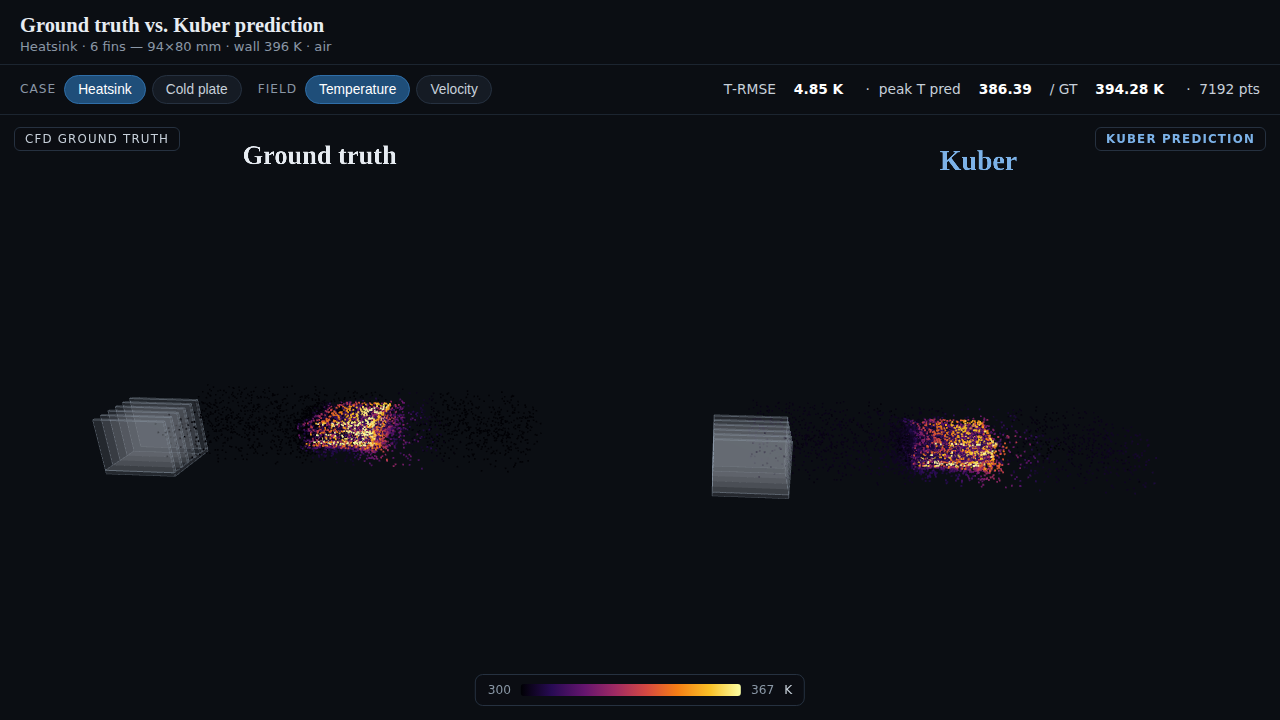
\includegraphics[width=0.98\textwidth]{gtvspred.png}
\caption{Qualitative comparison from the interactive viewer: solid device geometry with the fluid
temperature field, CFD ground truth (left) beside the surrogate prediction (right) for a heatsink;
peak-temperature and per-case $T$-RMSE are reported live.}
\label{fig:gtpred}
\end{figure*}

\subsection{Value of the self-generated corpus}
Does pretraining on the corpus help beyond the benchmark's own training set? A controlled A/B with the
same model and SIMSHIFT fine-tuning, changing only the initialization (Table~\ref{tab:vod}).
Pretraining helps materially at the easy shift ($-19\%$) and in-distribution ($-12\%$), modestly at
medium, and is neutral at the hardest shift, which the corpus does not yet cover. The only changed
ingredient is the corpus.

\begin{table}[t]\centering\small
\caption{Temperature RMSE (K); from scratch vs. corpus-pretrained then fine-tuned.}\label{tab:vod}
\begin{tabular}{@{}lccc@{}}\toprule
Shift & from scratch & pretrained & $\Delta$ \\ \midrule
easy & 8.99 & \textbf{7.28} & $-19\%$ \\
medium & 12.94 & \textbf{12.38} & $-4.3\%$ \\
hard & 14.42 & 14.43 & $\pm 0$ \\
in-dist. & 4.63 & \textbf{4.09} & $-12\%$ \\ \bottomrule
\end{tabular}
\end{table}

\subsection{Numerical stability}\label{sec:stab}
A deployable surrogate must reproduce steep near-wall gradients without over-smoothing or emitting
unphysical spikes. We measure the ratio of predicted to CFD temperature-gradient magnitude in the
edge band and at the steepest peaks (Table~\ref{tab:stab}). Every ratio is at or below unity, in and
out of distribution --- the surrogate never produces a steeper-than-physical gradient --- with an
explosion fraction of exactly zero and no NaN/Inf. It is not merely over-smoothing: the in-distribution
edge ratio ($0.97\approx1.0$) reproduces the true edge structure, while out of distribution it errs
slightly conservative, the safe direction.

\begin{table}[t]\centering\small
\caption{Predicted/CFD temperature-gradient ratio at edges (1.0 = faithful).}\label{tab:stab}
\begin{tabular}{@{}lcc@{}}\toprule
Metric & in-dist. & OOD \\ \midrule
edge-band $\nabla T$ ratio & 0.969 & 0.746 \\
steepest-peak (p99.9) ratio & 0.938 & 0.725 \\
explosion fraction & 0 & 0 \\
NaN / Inf count & 0 & 0 \\ \bottomrule
\end{tabular}
\end{table}

\subsection{Speed and data fidelity}
Inference is a single forward pass whose cost is independent of geometry, unlike CFD whose cost grows
with mesh size. Against measured OpenFOAM solve times (median 22 minutes, up to 117 for fine
geometries), a sub-second forward pass is roughly three to four orders of magnitude faster; we report
the inference figure as an estimate pending exact per-GPU timing. On fidelity, three prism boundary
layers recover the near-wall hot spot to within 0.1\,K of a fine mesh (378.8 vs.\ 378.9\,K) at
$\approx$2.7$\times$ fewer cells.

\section{Discussion and limitations}
We state the boundaries plainly. The corpus is air-dominated (tens of oil/glycol cases), so the model
is strongest on air. On SIMSHIFT the OOD axis is fin count alone; leave-one-fluid-out and
leave-one-shape-out remain future work. Cold plates are currently straight-channel, so the
multi-geometry result shows device-class generality rather than topology extrapolation. On the
averaged-nRMSE selector our temperature lead is bought with slightly higher velocity and pressure
error, reported transparently. Inference latency is an estimate. The multi-geometry numbers are on our
own corpus and are not comparable to the public benchmark.

\section{Conclusion}
Kuber packages the full stack needed to build a CHT surrogate --- a reproducible data engine, a
geometry-general surface-conditioned transformer, and an honest evaluation harness --- and
demonstrates it on electronics cooling, reaching state of the art on a public benchmark without domain
adaptation and spanning two device classes from one model. The same interfaces target the broader
class of coupled fluid--heat problems. Calibrated uncertainty, CAD connectors, and agentic geometry
optimization are natural next steps; code, data, and an interactive viewer are released to support
them.

\begin{thebibliography}{99}\small
\bibitem{pointnet} C.\,R. Qi, H. Su, K. Mo, L.\,J. Guibas. PointNet: Deep Learning on Point Sets for 3D Classification and Segmentation. \emph{CVPR}, 2017.
\bibitem{simshift} P. Setinek et al. SIMSHIFT: A Benchmark for Distribution Shift in Engineering Simulation. Preprint, 2025.
\bibitem{transolver} H. Wu, H. Luo, H. Wang, J. Wang, M. Long. Transolver: A Fast Transformer Solver for PDEs on General Geometries. \emph{ICML}, 2024.
\bibitem{upt} B. Alkin, A. F\"urst, S. Schmid, L. Gruber, M. Holzleitner, J. Brandstetter. Universal Physics Transformers. \emph{NeurIPS}, 2024.
\bibitem{abupt} B. Alkin et al. Anchored/Branched Universal Physics Transformers. Preprint, 2025.
\bibitem{fno} Z. Li, N. Kovachki, K. Azizzadenesheli, B. Liu, K. Bhattacharya, A. Stuart, A. Anandkumar. Fourier Neural Operator for Parametric PDEs. \emph{ICLR}, 2021.
\bibitem{deeponet} L. Lu, P. Jin, G. Pang, Z. Zhang, G.\,E. Karniadakis. Learning nonlinear operators via DeepONet. \emph{Nature Machine Intelligence}, 2021.
\bibitem{gino} Z. Li et al. Geometry-Informed Neural Operator for Large-Scale 3D PDEs. \emph{NeurIPS}, 2023.
\bibitem{pderefiner} P. Lippe, B. Veeling, P. Perdikaris, R. Turner, J. Brandstetter. PDE-Refiner: Achieving Accurate Long Rollouts with Neural PDE Solvers. \emph{NeurIPS}, 2023.
\bibitem{physicsnemo} NVIDIA. PhysicsNeMo: a framework for physics-ML (GeoTransolver). Software, Apache-2.0.
\bibitem{adam} D.\,P. Kingma, J. Ba. Adam: A Method for Stochastic Optimization. \emph{ICLR}, 2015.
\bibitem{weller} H.\,G. Weller, G. Tabor, H. Jasak, C. Fureby. A tensorial approach to computational continuum mechanics using object-oriented techniques. \emph{Computers in Physics}, 12(6), 1998.
\end{thebibliography}

\end{document}
